\documentclass[titlepage,10pt,openany]{scrbook}
\usepackage[papersize={107.5mm,148.5mm},twoside,bindingoffset=0.5cm,hmargin={1cm,1cm},
				vmargin={1.5cm,1.5cm},footskip=0.5cm,driver=dvipdfm]{geometry}
\usepackage[utf8]{inputenc}
\usepackage{graphicx}
\usepackage{wrapfig}
\usepackage[bahasa]{babel}
\usepackage{fancyhdr}
\usepackage{microtype}
\usepackage{pst-text}
\usepackage{palatino}
\usepackage{marvosym}
\usepackage{pdfpages}
\usepackage{hyphenat}

\renewcommand{\footrulewidth}{0.5pt}
\lhead[\fancyplain{}{\thepage}]%
      {\fancyplain{}{\rightmark}}
\rhead[\fancyplain{}{\leftmark}]%
      {\fancyplain{}{\thepage}}
\pagestyle{fancy}

\lfoot[\emph{\footnotesize Misa Peringatan 1 tahun \namaalm}]{}
\rfoot[]{\emph{\footnotesize Misa Peringatan 1 tahun \namaalm}}
\cfoot{}

\makeatletter
\newcommand{\judul}[1]{%
  {\parindent \z@ \centering 
    \interlinepenalty\@M \Large \bfseries #1\par\nobreak \vskip 20\p@ }}
\newcommand{\subjudul}[1]{%
  {\parindent \z@ 
    \interlinepenalty\@M \bfseries #1\par\nobreak \vskip 10\p@ }}
\newcommand{\lagu}[1]{%
  {\parindent \z@ 
    \interlinepenalty\@M \slshape \bfseries \normalsize \textit{#1}\par\nobreak \vskip 10\p@ }}
\newcommand{\keterangan}[1]{%
  {\parindent \z@  \slshape 
    \interlinepenalty\@M \textsl{#1}\par\nobreak  \vskip 5\p@}}

\renewenvironment{description}
               {\list{}{\labelwidth\z@ \itemindent-\leftmargin
                        \let\makelabel\descriptionlabel}}
               {\endlist}
\renewcommand*\descriptionlabel[1]{\hspace\labelsep 
                                \normalfont\bfseries #1 }


\makeatother

\newcommand{\BU}[1]{\begin{itemize} \item[U:] #1 \end{itemize}}
\newcommand{\BI}[1]{\begin{itemize} \item[I:] #1 \end{itemize}}
\newcommand{\BIU}[1]{\begin{itemize} \item[I+U:] #1 \end{itemize}}
\newcommand{\BPU}[1]{\begin{itemize} \item[P+U:] #1 \end{itemize}}
\newcommand{\BP}[1]{\begin{itemize} \item[P:] #1 \end{itemize}}
\newcommand{\inputlagu}[1]{\itshape{\input{#1}}}
\newcommand{\namaalm}{Bapak Vincentius Fererius Parlan }
\newcommand{\namaromo}{Rm. F.X. Tri Priyo Widarto SCJ}

\title{Misa Peringatan 1 Tahun}
\author{\namaalm}
\date{oleh \\ Rm \namaromo\\4 Juni 2016}
\hyphenation{sa-u-da-ra-ku}
\hyphenation{ke-ri-ngat}
\hyphenation{je-ri-tan}
\hyphenation{hu-bung-an}
\hyphenation{me-nya-dari}
\hyphenation{Eng-kau}
\hyphenation{ke-sa-lah-an}
\hyphenation{ba-gai-ma-na}
\hyphenation{Tu-han}
\hyphenation{di-per-ca-ya-kan}
\hyphenation{men-ja-uh-kan}
\hyphenation{bu-kan-lah}
\hyphenation{per-sa-tu-kan-lah}
\hyphenation{ma-khluk}
\hyphenation{Sem-buh-kan-lah}
\hyphenation{ja-lan}
\hyphenation{mem-bu-tuh-kan}
\hyphenation{be-ri-kan-lah}
\hyphenation{me-ra-sa-kan}
\hyphenation{te-man-ilah}
\hyphenation{mem-bi-ngung-kan}
\hyphenation{di-ka-gum-i}
\hyphenation{ta-ngis-an-Mu}
\hyphenation{mi-lik-ilah}

\DeclareFixedFont{\PT}{T1}{ppl}{b}{it}{0.5in}
\DeclareFixedFont{\PTsmall}{T1}{ppl}{b}{it}{0.2in}
\DeclareFixedFont{\PTsmallest}{T1}{ppl}{b}{it}{0.15in}
\DeclareFixedFont{\PTtext}{T1}{ppl}{b}{it}{11pt}
\DeclareFixedFont{\Logo}{T1}{pbk}{m}{n}{0.3in}

\hyphenation{me-nyi-ap-kan pan-jat-kan se-jah-te-ra Par-lan o-rang bang-kit}
\begin{document}
%\maketitle
\thispagestyle{empty}
%\begin{pspicture}(8cm,10cm)
%\psset{unit=1cm}
%\rput[cb](4,10){\PTsmall {EKARISTI}}
%\rput[cb](4,9){\PTsmall {PERINGATAN 100 HARI}}
%\rput[cb](4,8){\PTsmall {\namaalm}}
%\rput[cb](4,3){\PTsmallest {oleh}} 
%\rput[cb](4,2.5){\PTsmallest {Rm \namaromo}}
%\rput[cb](4,1){\PTsmallest {27 September 2015}}
%\end{pspicture}

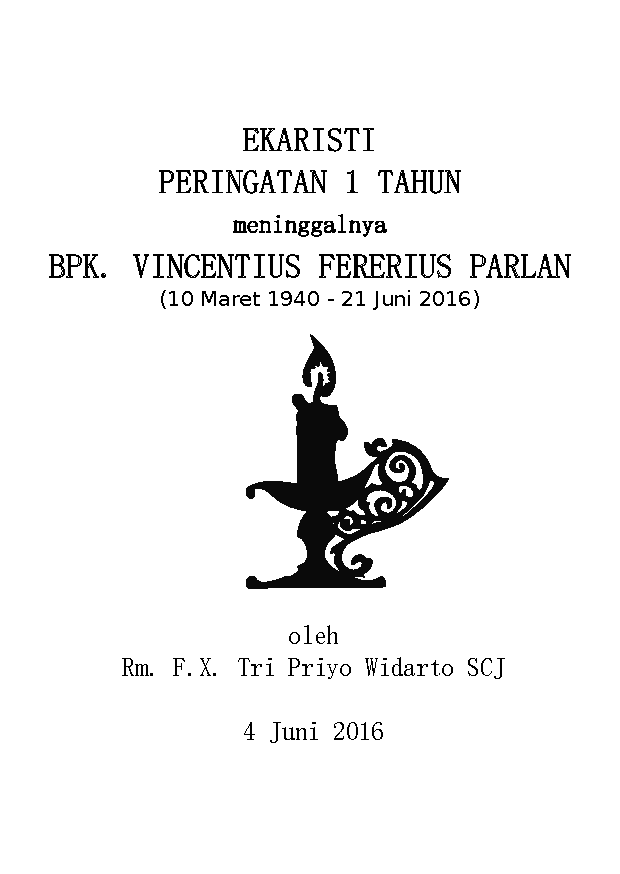
\includepdf{misa-1-tahun-vfp-cover}

\section*{RITUS PEMBUKA} 

 

\lagu{Lagu Pembuka}  
\small
\begin{center}
\itshape{Hatiku Percaya}
\end{center}


\begin{verse}
\itshape{
Saat ku tak melihat jalanMu\\
Saat ku tak mengerti rencanaMu\\
Namun tetap ku pegang janjiMu\\
Pengharapanku hanya padaMu\\
{~}\\
Saat ku tak melihat jalanMu\\
Saat ku tak mengerti rencanaMu\\
Namun tetap ku pegang janjiMu\\
Pengharapanku hanya padaMu\\
{~}\\
Reff :\\
Hatiku percaya, hatiku percaya\\
Hatiku percaya, s'lalu ku percaya\\
{~}\\
Lord I will trust in You\\
Lord I will trust in You\\
Lord I will trust in You\\
My heart will trust in You
}
\end{verse}
\normalsize 

\subjudul{Tanda Salib} 

\BI{Demi nama  Bapa dan Putera dan Roh Kudus}

\BU{Amin}

 

\subjudul{Salam}

\BI{Semoga kasih karunia, rahmat dan damai sejahtera dari 
Allah Bapa dan dari PuteraNya Yesus Kristus beserta 
saudara.} 

\BU{Sekarang dan selama-lamanya.}

 

\subjudul{Pengantar}

\BI{Saudara-saudari terkasih,
Hari ini kita bersama-sama berdoa bersama untuk
mendoakan arwah dari saudara kita \textbf{\namaalm} yang sudah satu tahun
yang lalu di panggil Bapa. Kita percaya bahwa segala
doa yang kita panjatkan untuk mereka yang sudah
meninggal sangat bermanfaat demi terwujudnya harapan
iman mereka untuk berdiam di rumah Tuhan selama-lamanya.}


\subjudul{Tobat}

\BI{Saudara-saudara, menyadari bahwa kita hanyalah serupa 
debu bernoda di depan alas kaki Allah Bapa, marilah kita 
bersyukur bahwa kita masih diperkenankan berdoa dan 
bermohon kepada Allah Bapa. 

Saya mengaku, \ldots \ldots
} 



\BI{Semoga Allah Bapa yang Maha Kuasa, mengasihani kita, 
mengampuni dosa kita dan mengantar kita ke dalam 
kehidupan kekal.}

\BU{Amin}

\lagu{Tuhan Kasihanilah Kami} 

\subjudul{Doa Pembuka}

\BI{Marilah berdoa\\
	Allah Bapa sumber sukacita, kami telah menerima jaminan kebahagiaan abadi dalam Diri Yesus Kristus Putera-Mu. Kami serahkan hamba-Mu, \namaalm{} yang telah Engkau panggil satu tahun yang lalu dalam sukacita surgawi. Persatukanlah kami dalam pengharapan akan kebahagiaan kekal di surga, kendati masih harus berjuang di dunia ini. Bantulah kami agar memiliki sukacita sejati dan saling menghibur satu sama lain. Dengan pengantaraan Yesus Kristus PuteraMu Tuhan kami yang bersama dengan Dikau dalam persekutuan Roh Kudus hidup dan berkuasa, Allah sepanjang segala masa.}

\BU{Amin}

 

\section*{LITURGI SABDA} 

\keterangan{Pembacaan dari Surat Paulus kepada umat di
Roma (Rom 8:9-15)}

\BP{Tetapi kamu tidak hidup dalam daging, melainkan dalam Roh, jika memang Roh Allah diam di dalam kamu. Tetapi jika orang tidak memiliki Roh Kristus, ia bukan milik Kristus.

Tetapi jika Kristus ada di dalam kamu, maka tubuh memang mati karena dosa, tetapi roh adalah kehidupan oleh karena kebenaran.
Dan jika Roh Dia, yang telah membangkitkan Yesus dari antara orang mati, diam di dalam kamu, maka Ia, yang telah membangkitkan Kristus Yesus dari antara orang mati, akan menghidupkan juga tubuhmu yang fana itu oleh Roh-Nya, yang diam di dalam kamu.

Jadi, saudara-saudara, kita adalah orang berhutang, tetapi bukan kepada daging, supaya hidup menurut daging.
Sebab, jika kamu hidup menurut daging, kamu akan mati; tetapi jika oleh Roh kamu mematikan perbuatan-perbuatan tubuhmu, kamu akan hidup.

Semua orang, yang dipimpin Roh Allah, adalah anak Allah.
Sebab kamu tidak menerima roh perbudakan yang membuat kamu menjadi takut lagi, tetapi kamu telah menerima Roh yang menjadikan kamu anak Allah. Oleh Roh itu kita berseru: "ya Abba, ya Bapa!"

Demikianlah Sabda Tuhan.}

\BU{Syukur kepada Allah}

 

\lagu{Lagu tanggapan sabda}
\small
\begin{center}
\itshape{Keheningan hati}
\end{center}

\begin{verse}
\itshape{
Di sela hening hati ini\\
Ku dengar sabdaMu ya Tuhan\\
Menggema lembut dalam kalbu\\
Membuka mata hatiku\\
{~}\\
\textbf{Ref:}\\
Ku ingin melangkah seturut sabdaMu\\
Agar ku selalu dekat denganMu\\
Kan ku wartakan sabdaMu Tuhan\\
Ke seluruh penjuru dunia\\
{~}\\
Ajarku tuk selalu setia,\\
Menjadi saksi dan pewarta,\\
Hingga di seluruh dunia, \\
MemujiMu, Alleluya 
}
\end{verse}
\normalsize

 

\subjudul{Injil}

\BI{Tuhan sertamu}

\BU{dan sertamu juga} 

\BI{Inilah Injil Yesus Kristus menurut Lukas (4:16-22a)}

\BU{Dimuliakanlah Tuhan}

\BI{Ia datang ke Nazaret tempat Ia dibesarkan, dan menurut kebiasaan-Nya pada hari Sabat Ia masuk ke rumah ibadat, lalu berdiri hendak membaca dari Alkitab.
Kepada-Nya diberikan kitab nabi Yesaya dan setelah dibuka-Nya, Ia menemukan nas, di mana ada tertulis:
"Roh Tuhan ada pada-Ku, oleh sebab Ia telah mengurapi Aku, untuk menyampaikan kabar baik kepada orang-orang miskin; dan Ia telah mengutus Aku
untuk memberitakan pembebasan kepada orang-orang tawanan, dan penglihatan bagi orang-orang buta, untuk membebaskan orang-orang yang tertindas, untuk memberitakan tahun rahmat Tuhan telah datang."

Kemudian Ia menutup kitab itu, memberikannya kembali kepada pejabat, lalu duduk; dan mata semua orang dalam rumah ibadat itu tertuju kepada-Nya.
Lalu Ia memulai mengajar mereka, kata-Nya: "Pada hari ini genaplah nas ini sewaktu kamu mendengarnya." Dan semua orang itu membenarkan Dia dan mereka heran akan kata-kata yang indah yang diucapkan-Nya, lalu kata mereka: "Bukankah Ia ini anak Yusuf?"
}


\BI{Demikianlah Injil Tuhan}

\BU{Terpujilah Kristus}

 

\subjudul{Homili}

\subjudul{Syahadat} 

\subjudul{Doa Umat}

\BI{Saudara-saudari, kehadiran kita bersama di sini adalah untuk mengungkapkan iman kita akan Allah sumber sukacita sejati. Marilah dengan rendah hati kita ungkapkan doa dan permohonan kita kepada Bapa:}
% % %
\BP{Bagi saudara kita \textbf{\namaalm} yang sudah dipanggil Bapa 1 
tahun yang lalu. Semoga melalui pembaptisan yang telah
diterima saudara kita \textbf{\namaalm} dan berkat iman akan Yesus
sepanjang hidupnya, ia dianugerahi hidup kekal yang
telah dijanjikan Allah sendiri kepadanya.

\textit{Hening sejenak \ldots\ldots} 

Marilah kita mohon :}

\BU{Kabulkanlah doa kami ya Tuhan}


\BP{Di kala hidup, saudara kami \namaalm{} telah berusaha mengabdi kepada-Mu dengan sebaik-baiknya. 
Tetapi karena kelemahannya, saudara kami ini sering melukai hatiMu yang Kudus. Oleh karena itu kami mohon 
sudilah kiranya Engkau mengampuni segala dosanya hingga ia pantas menghadap-Mu. 

\textit{Hening sejenak \ldots\ldots} 

Marilah kita mohon :}

\BU{Kabulkanlah doa kami ya Tuhan.}

\BP{Bagi orang-orang yang telah meninggal dan
yang masih mengharapkan belah kasihan Allah.
Semoga, berkat belas kasihan dan kerahimanNya,
Allah  memberikan pengampunan kepada
mereka semua, sehingga mereka boleh beristirahat dalam kebahagiaan abadi bersama Bapa
di surga. 

\textit{Hening sejenak \ldots\ldots} 

Marilah kita mohon :}

\BU{Kabulkanlah doa kami ya Tuhan.}

\BP{Bagi kami yang hadir dalam peringatan ini.
Semoga kami lebih menyadari bahwa Engkau menghendaki semua orang mendapatkan kebahagiaan
hidup di dalam kemuliaan-Mu.
Semoga kami yang telah mendengarkan dan merenungkan sabda Tuhan, juga mampu mengimani
janji Yessus Kristus, yang terwujud dalam perjuangan hidup dan karya kami sehari-hari.

\textit{Hening sejenak \ldots\ldots} 

Marilah kita mohon :}

\BU{Kabulkanlah doa kami ya Tuhan.}


\BI{Bapa kasihMu tiada batas, kesabaranMu begitu besar. Semoga dalam pengharapan iman yang benar, kami senantiasa dalam limpahan rahmat-Mu, dengan pengantaraan Kristus Tuhan kami.}

\BU{Amin}

\section*{LITURGI EKARISTI}

\lagu{Lagu pengantar persembahan}
\small
\begin{center}
\itshape{T’rimalah Syukur Kami}
\end{center}

\begin{verse}
\itshape{
Trimalah, syukur kami, trimalah bakti kami.\\
Trimalah dalam tangan kasih-Mu.\\
Bersama anggur roti pralambang karya bakti\\
Trimalah dalam tangan kasih-Mu.\\
{~}\\
Berkatilah Tuhan, kuduskanlah Tuhan\\
dalam perjamuan ini,\\
agar menjadi satu dengan korban Putra-Mu\\
menjadi persembahan yang kudus.\\
{~}\\
Bukanlah emas perak, bukanlah intan berlian,\\
bukanlah permata nan mulia.\\
Hanyalah ketulusan, hanyalah kesetiaan\\
trimalah dalam tangan kasih-Mu.\\
{~}\\
Berkatilah Tuhan, kuduskanlah Tuhan\\
dalam perjamuan ini,\\
agar menjadi satu dengan korban Putra-Mu\\
menjadi persembahan yang kudus.
}
\end{verse}
\normalsize



\BI{Kami memuji Engkau ya Bapa, Allah semesta alam, sebab 
dari kemurahanMu kami menerima roti dan anggur yang 
kami persembahkan ini. Inilah hasil dari bumi dan usaha 
manusia yang bagi kami akan menjadi santapan rohani.}

\BU{Terpujilah Allah selama-lamanya}

\BI{Berdoalah saudara-saudara supaya persembahan kita ini 
diterima oleh Allah Bapa yang mahakuasa.}

\BU{Semoga persembahan ini diterima demi kemuliaan Tuhan 
dan keselamatan kita serta seluruh umat Allah yang kudus.}

\BI{Ya Allah Bapa di surga, pengampunanMu menjadi sumber 
kedamaian dan kekuatan baru di dalam hati kami untuk 
mengikuti PuteraMu dengan setia. Maka kami mohon 
pandanglah dengan rela persembahan di atas altar ini dan 
teguhkanlah hati kami berkat korban Yesus Kristus, Tuhan 
dan Pengantara kami kini dan sepanjang masa.}

\BU{Amin} 

\subjudul{DOA SYUKUR AGUNG}


\subjudul{Kudus}

\subjudul{Bapa Kami}

\subjudul{Anak Domba Allah}

\subjudul{Komuni}
\newpage
\subjudul{Lagu Komuni}
\small
\begin{center}
\itshape{S'perti Rusa Rindukan Sungai-Mu}
\end{center}


\begin{verse}
\itshape{
S'perti rusa rindukan sungai-Mu, \\
jiwaku rindu Engkau.\\
Kaulah Tuhan hasrat hatiku\\
kurindu menyembah-Mu\\
Engkau kekuatan dan perisaiku\\
kepada-Mu rohku berserah\\
Kaulah Tuhan hasrat hatiku\\
kurindu menyembah-Mu\\
Yesus, Yesus, Kau berarti bagiku\\
Yesus, Yesus, Kau segalanya bagiku\\
{~}\\
As the deer panteth for the waters,\\
so my soul longeth after Thee\\
You are Lord of all my heart desire\\ 
and I long to worship Thee.\\
You are my Lord of my strength and my shield, \\
to you a long may my spirit yield.\\
You are Lord of all my heart desire\\ 
and I long to worship Thee.\\
Jesus, Jesus You are everything for me\\
Jesus, Jesus You are everything for me
}
\end{verse}
\normalsize

 

\subjudul{Doa sesudah komuni}

\BI{Marilah berdoa: Terima kasih ya Allah, atas anugerah 
terbesar yaitu kami telah diberi rahmat untuk mengenal 
Yesus Kristus. Dalam Dia manusia yang berdosa mendapat 
pengampunan dan perlindungan. Semoga kami berani 
melepaskan semuanya dan menjadi serupa dengan Dia 
dalam kematianNya. Sebab Dialah Tuhan dan pengantara 
kami kini dan sepanjang masa.}

\BU{Amin.}

 

\section*{RITUS PENUTUP}

\BI{Tuhan beserta kita}

\BU{Sekarang dan selama-lamanya}

\BI{Semoga saudara sekalian diberkati oleh Allah Yang 
Mahakuasa \Cross ~Bapa dan Putera dan Roh Kudus.}

\BU{Amin}

 

\subjudul{Pengutusan}

\BI{Saudara sekalian, Perayaan Ekaristi untuk memohon 
berkat Allah Bapa bagi arwah \namaalm telah selesai.}

\BU{Syukur kepada Allah}

\BI{Kita diutus untuk mewartakan bahwa Tuhan Yesus adalah 
jalan, kebangkitan dan hidup.}

\BU{Amin.}

 

\lagu{Lagu Penutup}

\vspace{1cm}

\small
\begin{center}
\itshape{Asma Dalem Maria}
\end{center}


\begin{verse}
\itshape{
Asma dalem Mariyah,\\
damel trenyuh manah.\\
Mring pra putra Mariyah\\
ingkang setya tansah.\\
{~}\\
\textbf{Refren:}\\
Mugi asma Mariyah,\\
dumeling ing manah.\\
Yen amba tinimbalan,\\
nyuwun langgeng bingah.\\
{~}\\
Asma ingkang pinuji,\\
ing sagunging bangsa.\\
Asma paring prajanji\\
mring putra kang setya.\\
{~}\\
Yen amba nandhang susah,\\
nyuwun sihing lipur.\\
Asma dalem Mariyah\\
paring berkah luhur
}
\end{verse}
\normalsize

 

\newpage
\begin{flushright}
{\Large Ucapan terima kasih}\\
\noindent Dengan penuh syukur dalam kasih Tuhan, kami mengucapkan banyak
terima kasih kepada:
\large

\textbf{Romo \namaromo}\\
yang telah berkenan memimpin perayaan ekaristi peringatan 1 tahun meninggalnya\\ \namaalm
ini.

\textbf{Koor Calista}\\
yang telah menyemarakkan perayaan ekaristi ini.

\textbf{Umat lingkungan St. Yustinus, para undangan, segenap keluarga, dan orang-orang terkasih}\\
yang telah berkenan hadir memberikan cinta dan doa dalam perayaan
ekaristi ini.

Semoga Tuhan memberkati dan memelihara ikatan kasih\\ di antara kita semua.

Amin.

\bigskip 

\textit{Ibu MG Waldjijah\\
dan segenap keluarga}
\end{flushright}

\end{document} 

[07:09, 5/24/2016] +62 813-2829-0020: 
Pembk hatiku percaya, antar bacaan keheningan hati, persembahan terimalah syukur kami, Kom bagaikan rusa rindukan sungaimu, penutup Asmo Dalem Maria.
[07:09, 5/24/2016] +62 813-2829-0020: Lagu misa tgl 4 Juni, ordinarium Lauda sion

Undefined control sequence. Marilah kita mohon :}